\chapter{评价}
\label{cha:eval}
    我们的测试实验主要分为三部分,第一部分对调度预测进行测试,第二部分对性能模型进行测试,第三部分对整体模型进行测试。
    
\section{测试集}
    对第一部分测试和第三部分测试,我们采用自行创建的数据流图和现实存在的神经网络两类模型进行测试。
    
    自建数据包含三个测试:
    
    1. 级联测试:测试多个矩阵乘法级联的情况。\ref{fig:sche_cascade}所示。
    
    2. 并行测试:测试可以并行的计算节点的调度情况。如图\ref{fig:sche_parallel}所示。

    3. 资源测试:测试多个不同操作抢占硬件资源的情况。如图\ref{fig:sche_resource}所示。

    \begin{figure}[!htbp]
        \centering
        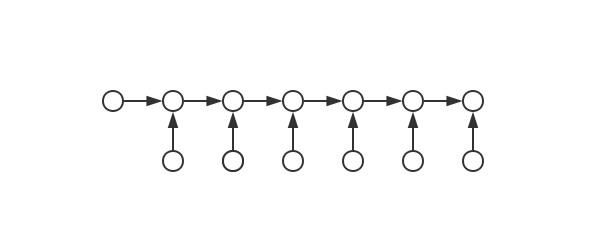
\includegraphics[width=0.8\textwidth]{figures/sche_cascade.jpg}
        \caption{级联测试数据流图示意图}
        \label{fig:sche_cascade}
    \end{figure}

    \begin{figure}[!htbp]
        \centering
        \begin{minipage}[t]{0.4\textwidth}
            \centering
            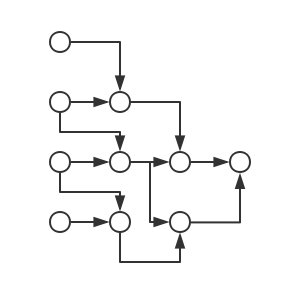
\includegraphics[width=1\textwidth]{figures/sche_parallel.jpg}
            \caption{并行测试数据流图示意图}
            \label{fig:sche_parallel}
        \end{minipage}
        \begin{minipage}[t]{0.4\textwidth}
            \centering
            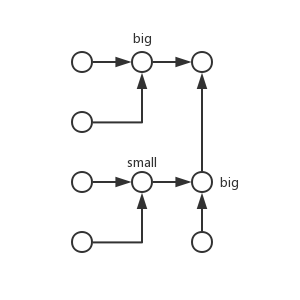
\includegraphics[width=1\textwidth]{figures/sche_resource.jpg}
            \caption{资源测试数据流图示意图}
            \label{fig:sche_resource}
        \end{minipage}
    \end{figure}

    神经网络测试包含两个测试:
    
    1. LeNet-5:作为规模较小的卷积神经网络,如图\ref{fig:lenet5_str}。

    \begin{figure}[!htbp]
        \centering
        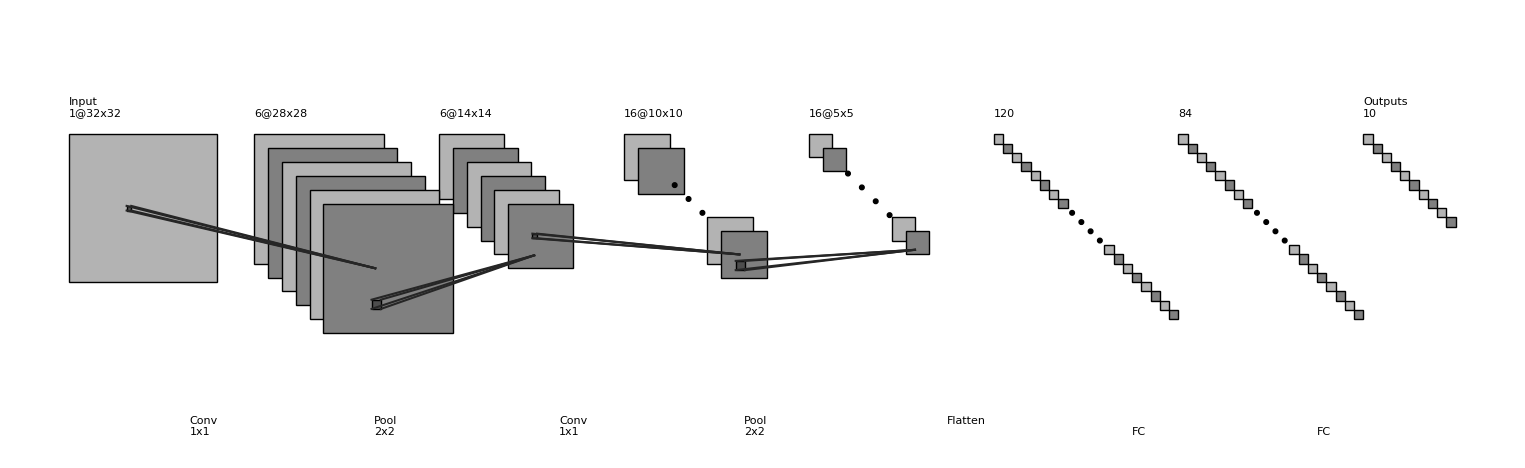
\includegraphics[width=0.8\textwidth]{figures/lenet5_str.png}
        \caption{LeNet-5示意图}
        \label{fig:lenet5_str}
    \end{figure}
    
    2. AlexNet:作为规模较大的卷积神经网络,如图\ref{fig:alexnet_str}

    \begin{figure}[!htbp]
        \centering
        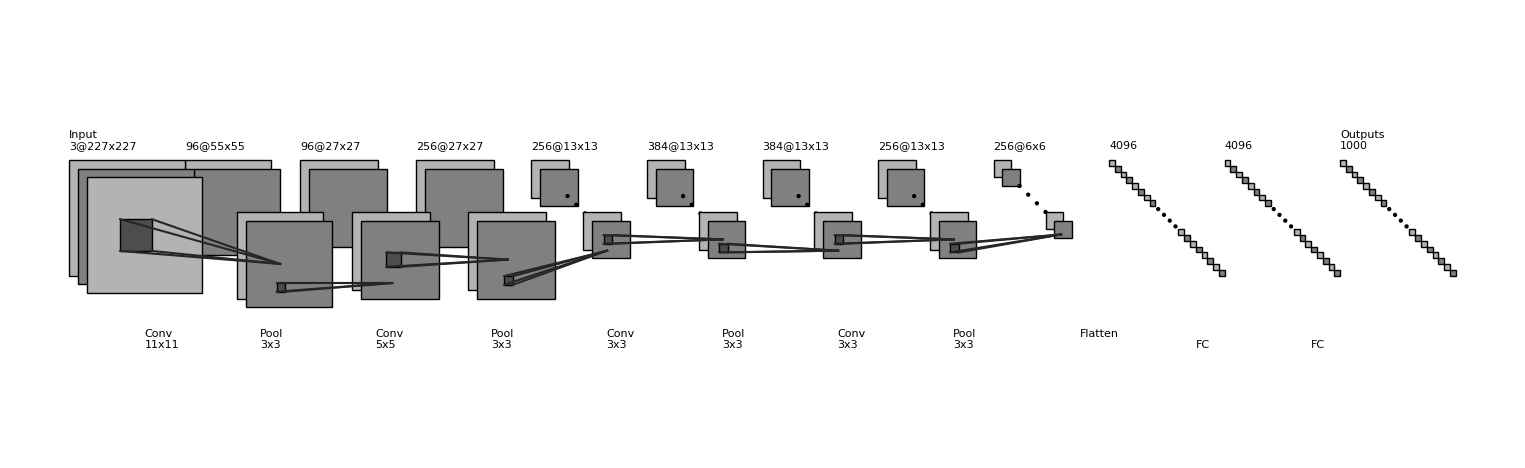
\includegraphics[width=0.8\textwidth]{figures/alexnet_str.png}
        \caption{AlexNet示意图}
        \label{fig:alexnet_str}
    \end{figure}
    
    由于卷积神经网络的结构没有较为大的变化,因此选取这两个测试可以较好的说明我们的模型的预测能力。

\section{调度预测}
    这一节我将针对调度预测模块进行测试。我们的目标是测试调度模拟能够多大程度恢复任务真实的运行状况。因此,我们的测试方法是,首先正常运行测试,拿到测试的时间轴数据,得到每个节点的运行时间。之后将这一数据作为性能模型代入调度模拟器。这时用得到的预测结果和实际运行时间进行比较,就可以说明调度模拟器的性能。
    
    由于GPU运行时,我们无法通过时间轴数据拿到在一次运行中每个操作的运行时间,我们在这一节测试中仅对CPU数据进行测试。数据如表\ref{tab:sche}所示。我们可以看到,我们的预测结果和实际运行时间的相对偏差均小于10\%。可以很好地模拟实际TensorFlow的调度过程。
    
    \begin{table}[!htbp]
        \centering
	    \caption{调度模型测试结果}
        \label{tab:sche}
        \begin{tabular}{|l|l|l|l|l|}
            \hline
            测试名称 & 运行时间(s) & 预测时间(s) & 相对偏差 & 数据偏差\\
            \hline
            矩阵级联 & 0.423 & 0.416 & 1.65\% & 0.41\% \\
            \hline
            并行调度 & 0.412 & 0.405 & 1.70\% & 0.59\% \\
            \hline
            资源调度 & 0.244 & 0.238 & 2.5\% & 0.21\% \\
            \hline
            LeNet-5 & 0.149 & 0.142 & 4.7\% & 0.38\% \\
            \hline
            AlexNet & 1.53 & 1.45 & 5.2\% & 7.2\% \\
            \hline
        \end{tabular}
    \end{table}
    
    另一方面,TensorFlow的会话启动需要时间,通过会话启动图也需要时间,因此实际预测流程应该增加一个常数项,用来模拟这部分时间。我们的实验中,我们认为我们的运行结果已经足够支持后续的工作,因此没有单独对这一部分进行分析。
    
\section{性能模型}
    本节我们将对所有性能模型模块分别进行测试。我们对每一个模块,随机生成若干组测试数据。对每组测试数据测量实际运行时间,再通过对应的性能模型生成预测时间。将两者进行对比,评估性能模型的准确程度。
    
    在\ref{sec:impl_model}章,我们对性能模型有一定的讨论,在数据规模较小的时候,测试过程本身带来的误差有可能和实际运行时间在同一个数量级。因此,性能模型中不可避免地有一部分明显不符合模型的数据,这类数据我们称为异常点。在我们的评价中,我们将相对偏差在$ -50\% $到$ +100\% $以外的数据作为异常点处理。这一部分数据我们将在计算准确度的时候舍弃掉,并将异常点个数作为评价模型的指标之一。
    
    其他数据我们选取平均相对偏差作为评价指标。平均相对偏差的公式如下:
    
    $$
        \bar{\delta} = \frac{\sum_{i=1}^N abs(x_i - \mu_i)}{N}
    $$
    
    选取平均相对偏差的好处在于,可以清楚的观察到预测数据和真实数据的差距,较为直观。整体测试结果如表\ref{tab:model}所示。下面我将对每个模型的数据进行分析。

    \begin{table}[!htbp]
        \centering
	    \caption{性能模型测试结果}
        \label{tab:model}
        \begin{tabular}{|l|l|l|l|}
            \hline
            测试名称 & 异常点数量 & 平均相对偏差 & 模型质量 \\
            \hline
            MatMul(CPU) & 6 & 12.0\% & 好 \\
            \hline
            MatMul(GPU) & 0 & 11.5\% & 非常好 \\
            \hline
            Conv2D(GPU) & 13 & 20.3\% & 中等 \\
            \hline
            Conv2D(CPU) & - & 87\% & 不好 \\
            \hline
            LRN(CPU) & 9 & 18.7\% & 好 \\
            \hline
            LRN(GPU) & 0 & 18.4\% & 非常好 \\
            \hline
        \end{tabular}
    \end{table}

\subsection{矩阵乘法}
    我们在CPU上测试了随机的128个不同规模的矩阵乘法,这部分测试中,异常点有6个。这6个点均为规模非常小,运行时间比较短的情况。我们的模型在这类数据中会倾向于将时间预测长几个毫秒。这种情况的发生,可能时因为在TensorFlow中不同规模的计算采用了不同的实现,导致初始化时间不一致带来的模型拟合过程中的误差。这类数据由于绝对误差并不大,因此对我们进行矩阵乘法的预测不会带来过大影响。
    
    我们在CPU上的矩阵乘法预测模型,平均相对偏差达到12.0\%,可以很好的满足我们的模型使用需求。有趣的是,在结果统计中,我们发现,我们的模型中预测值大于实际值的比例达到68\%,因此,在后续的优化中,我们可以通过增加常数项或系数的方式进行修正。

    在GPU上,我们同样测试了128个数据点,而这128组测试中没有异常点。同时,平均相对偏差达到11.5\%,因此GPU上的矩阵乘法模型是一个较为准确而且稳定的模型。

\subsection{二维卷积}
    我们在CPU上测试了随机的128个不同规模的二维卷积操作。这部分测试中,异常点有13个,这些点的绝对偏差值均为毫秒级别,因此不会对模型带来过大的影响。
    
    在去除掉离群点后,平均相对偏差为20.3\%可以基本满足我们的预测需求。

    而在GPU上,我们的预测模型性能不佳,仅能保证数量级上的一致,所有数据的平均相对偏差为87\%。但由于由于预测数据和实际数据差别基本在$ -50\% $到$ +100\% $之间,因此这一测试模型依然可以帮助我们进行分析。
    
    正如我们在\ref{ssec:impl_conv}中所讨论的,GPU上二维卷积运算优化方式较多,实际运行情况由于动态调度问题的存在,运行时间也不稳定。因此,不同规模的二维卷积底层进行的函数调用是不同的,因此,我认为,针对这个操作,可能需要函数调用的粒度才能比较好地预测运行时间,而这样就需要动态的运行信息,和我们的设计初衷不一致,因此我们在GPU上二维卷积的预测目前阶段只能达到这一步。

\subsection{局部响应归一化}
    我们在CPU上测试了随机的128个不同规模的局部响应归一化操作。这部分测试中,异常点有9个,均为小规模数据,而且相对偏差不超过200\%,对模型影响较小。
    
    去除掉离群点后,平均相对偏差为18.7\%。能够比较好地满足我们的使用需求。
    
    在GPU上的测试中,没有离群点的出现,所有数据的平均相对偏差为18.4\%,可以基本满足我们的需求。

\section{综合预测}
    在这一节,我们将对模型整体表现进行评估,测试数据沿用第一节所介绍的方法。我们对每个测试模型使用完整的性能模型进行预测,和第二节中得到的模型真实运行时间进行对比,评价整体模型的准确程度,测试结果如表\ref{tab:pre_cpu}和表\ref{tab:pre_gpu}所示。
    
    \begin{table}[!htbp]
        \centering
	    \caption{CPU上综合测试结果}
        \label{tab:pre_cpu}
        \begin{tabular}{|l|l|l|l|}
            \hline
            测试名称 & 运行时间(s) & 预测时间(s) & 相对偏差(s)\\
            \hline
            矩阵级联 & 0.423 & 0.419 & 0.95\% \\
            \hline
            并行调度 & 0.412 & 0.419 & 1.70\% \\
            \hline
            资源调度 & 0.244 & 0.247 & 1.70\% \\
            \hline
            LeNet-5 & 0.149 & 0.157 & 5.37\% \\
            \hline
            AlexNet & 1.53 & 1.90 & 24.2\% \\
            \hline
        \end{tabular}
    \end{table}
    
    \begin{table}[!htbp]
        \centering
	    \caption{GPU上综合测试结果}
        \label{tab:pre_gpu}
        \begin{tabular}{|l|l|l|l|}
            \hline
            测试名称 & 运行时间(ms) & 预测时间(ms) & 相对偏差\\
            \hline
            矩阵级联 & 19.96 & 24.57 & 23.1\% \\
            \hline
            并行调度 & 24.38 & 24.57 & 0.779\% \\
            \hline
            资源调度 & 13.29 & 14.83 & 11.6\% \\
            \hline
            LeNet-5 & 62.47 & 29.04 & 53.5\% \\
            \hline
            AlexNet & 116.6 & 217.4 & 86.45\% \\
            \hline
        \end{tabular}
    \end{table}
    
    我们可以看到,在三项自定义测试中,由于操作选取较为规整,对应的模型结果较为准确,因此能够比较好的还原运行状况。而在卷积神经网络测试中,尽管结果不如自定义测试,依然能够较好地还原运行时间数据。
    
    另一方面,CPU上我们的预测模型准确度要优于GPU,原因是GPU上二维卷积操作模型不够准确,拉低了整体的准确度。

\section{多GPU测试}
    为了较好地验证模型预测多GPU性能的正确性。我们仅对三个自定义数据集进行测试。在这部分测试中,我们为了更为数据更为精准,以便验证多GPU部分,我们加大了数据规模,使每个操作的时间拉长。测试结果如表\ref{tab:mul_gpu}所示。
    
    \begin{table}[!htbp]
        \centering
	    \caption{多GPU上测试结果}
        \label{tab:mul_gpu}
        \begin{tabular}{|l|l|l|l|}
            \hline
            测试名称 & 运行时间(ms) & 预测时间(ms) & 相对偏差\\
            \hline
            矩阵级联 & 124.2 & 126.22 & 1.46\% \\
            \hline
            并行调度 & 74.2 & 68.97 & 7.05\% \\
            \hline
            资源调度 & 54.4 & 54.86 & 0.85\% \\
            \hline
        \end{tabular}
    \end{table}
    
    我们可以看到,我们的模型在多GPU上能有比较好的运行结果,能够说明我们的模型在更为准确的性能模型下,能够有效地预测多GPU下深度神经网络的运行状况。
    
\section{对比实验}
    最后,我们将我们实现的预测模型和TensorFlow自带的cost\_analyzer工具进行对比,如表\ref{tab:cmp_cpu}和表\ref{tab:cmp_gpu}所示。
    
    我们可以看出,无论在CPU还是GPU上,我们的预测模型都明显优于TensorFlow自带的cost\_analyzer工具。在CPU中,我们的模型最高能将误差优化到原先的1.5\%,在GPU上,我们的模型最高能将误差优化到原先的1\%。
    
    因此,我们的预测模型能够比较好的完成对TensorFlow中深度神经网络的运行模拟。

    \begin{table}[!htbp]
        \centering
	    \caption{综合测试结果对比(CPU),其中预测时间为我们实现的性能模型的预测时间,分析时间为TensorFlow分析工具的预测时间}
        \label{tab:cmp_cpu}
        \begin{tabular}{|l|l|l|l|}
            \hline
            测试名称 & 运行时间(s) & 预测时间(s) & 分析时间(s)\\
            \hline
            矩阵级联 & 0.423 & 0.419 & 3.08 \\
            \hline
            并行调度 & 0.412 & 0.419 & 3.08 \\
            \hline
            资源调度 & 0.244 & 0.247 & 1.80 \\
            \hline
            LeNet-5 & 0.149 & 0.157 & 0.0046 \\
            \hline
            AlexNet & 1.53 & 1.90 & 7.77 \\
            \hline
        \end{tabular}
    \end{table}

    \begin{table}[!htbp]
        \centering
	    \caption{综合测试结果对比(GPU),其中预测时间为我们实现的性能模型的预测时间,分析时间为TensorFlow分析工具的预测时间}
        \label{tab:cmp_gpu}
        \begin{tabular}{|l|l|l|l|}
            \hline
            测试名称 & 运行时间(ms) & 预测时间(s) & 分析时间(ms)\\
            \hline
            矩阵级联 & 19.96 & 24.57 & 3.86 \\
            \hline
            并行调度 & 24.38 & 24.57 & 4.70 \\
            \hline
            资源调度 & 13.29 & 14.83 & 3.52 \\
            \hline
            LeNet-5 & 62.47 & 29.04 & 0.84 \\
            \hline
            AlexNet & 116.6 & 217.4 & 29.4 \\
            \hline
        \end{tabular}
    \end{table}